\documentclass[10pt,a4paper]{article}

\usepackage{afterpage}
\usepackage{pgfplots}
\usepackage{siunitx}
\usepackage{tikz}
\usepackage{amsmath}
\usepackage{amssymb}
\usepackage{nomencl}
\usepackage{url}
\usepackage{listings}
\usepackage{color}
\usepackage{caption}
\usepackage{subcaption}
\usepackage{float}
\usepackage[margin=1in]{geometry}
\usepackage{multirow}
\usepackage{graphicx}
\makenomenclature

\definecolor{dkgreen}{rgb}{0,0.6,0}
\definecolor{gray}{rgb}{0.5,0.5,0.5}
\definecolor{mauve}{rgb}{0.58,0,0.82}

\lstset{frame=tb,
	language=C++,
	aboveskip=3mm,
	belowskip=3mm,
	showstringspaces=false,
	columns=flexible,
	basicstyle={\small\ttfamily},
	numbers=none,
	numberstyle=\tiny\color{gray},
	keywordstyle=\color{blue},
	commentstyle=\color{dkgreen},
	stringstyle=\color{mauve},
	breaklines=true,
	breakatwhitespace=true,
	tabsize=3
}


\pgfplotsset{compat=newest} % Allows to place the legend below plot
\usepgfplotslibrary{units} % Allows to enter the units nicely

\sisetup{
	round-mode          = places,
	round-precision     = 2,
}

\numberwithin{equation}{section}

\makeindex

\pagenumbering{gobble}
\begin{document}
	
	\begin{titlepage}
		
		\newcommand{\HRule}{\rule{\linewidth}{0.5mm}} % Defines a new command for the horizontal lines, change thickness here
		
		\center % Center everything on the page
		
		\textsc{\LARGE Cranfield University}\\[1.5cm] % Name of your university/college
		\textsc{\Large Computational and Software Techniques in Engineering}\\[0.5cm] % Major heading such as course name
		\textsc{\large Gruop Project}\\[0.5cm] % Minor heading such as course title
		
		\HRule \\[0.4cm]
		{ \huge \bfseries Assignment}\\[0.4cm] % Title of your document
		\HRule \\[1.5cm]
		
		\begin{minipage}{0.4\textwidth}
			\begin{flushleft} \large
				\emph{Authors:}\\
				Benjamin \textsc{Deguerre}\\
				Wojciech \textsc{Jonczyk}\\ % Your name
				Alix \textsc{Kamano}\\
				Anna \textsc{Zaporowska}
			\end{flushleft}
		\end{minipage}
		~
		\begin{minipage}{0.4\textwidth}
			\begin{flushright} \large
				\emph{Supervisor:} \\
				Dr. Chi chun gilbert \textsc{Tang} % Supervisor's Name
			\end{flushright}
		\end{minipage}\\[2cm]
		
		{\large 10 December 2016}\\[3cm] % Date, change the \today to a set date if you want to be precise
		
		
\includegraphics{logo}\\[2cm] % Include a department/university logo - this will require the graphicx package
		
		
		\vfill % Fill the rest of the page with whitespace
		
	\end{titlepage}

\tableofcontents
\section{Introduction}
\begin{figure}[H]
	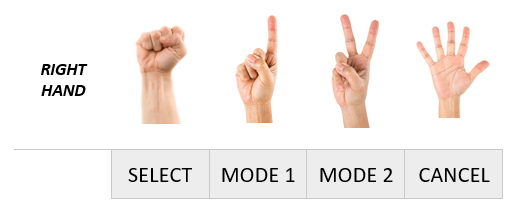
\includegraphics{mode_selection}
	\centering
	\caption{Mode selection - set of gestures}
	\label{fig:mode}
\end{figure}
\newpage

\chapter{Conclusion}

\newpage

\end{document}
